\documentclass[11pt]{article}

\usepackage[a4paper,margin=1in]{geometry}
\usepackage{times}
\usepackage{hyperref}
\usepackage{listings}
\usepackage{graphicx}
\usepackage{amsmath}
\usepackage{booktabs}

\title{Rabt: Computing Minimal Dependency Context for LLM-Based Code Intelligence}
\author{Muhammad Taha\\[4pt]\texttt{bolt.taha.work@gmail.com}
  \and Affan Khan\\[4pt]\texttt{affanghouri333@gmail.com}}
\date{}

\begin{document}

\maketitle

\begin{abstract}
Large Language Models (LLMs) have shown strong performance on function-level code generation, but repository-level software engineering remains challenging.
Current tools such as IDE copilots and retrieval-augmented generation (RAG) systems typically guess context using semantic search over files, which can miss critical dependencies and waste tokens on irrelevant code.
This paper presents \emph{Rabt}, a research-grade prototype that computes a hybrid static+runtime dependency graph for a codebase and extracts a minimal, high-signal subgraph as context for LLMs.
Rabt integrates (1) static analysis, (2) runtime tracing of calls and mutations, (3) impact scoring by execution frequency, (4) a query agent that traverses the graph to build minimal subgraphs, and (5) a change-detection pipeline that incrementally updates the graph using \texttt{git diff}.
On a real-world library (\texttt{requests}), Rabt answers the question ``Who calls \texttt{request}?'' using less than 1\% of the graph nodes, and on SWE-style scenarios it achieves up to 99.96\% context reduction (375k characters $\rightarrow$ 136 characters) while preserving answer correctness.
These results suggest that computing explicit dependency context can make high-intelligence reasoning models (e.g., OpenAI~o1) economically viable for mass-scale code analysis.
\end{abstract}

\section{Introduction}

Modern AI coding tools, such as Cursor and GitHub Copilot, rely heavily on semantic search, vector retrieval, and file-level heuristics to decide which code to show an LLM.
These methods \emph{guess} context: they often retrieve textually or semantically similar files, but they do not explicitly model the actual dependency structure of the program.
As repositories grow in size and complexity, this leads to \emph{context rot}: the LLM sees long, noisy prompts that omit crucial edges (e.g., hidden callers, runtime mutations) and include many irrelevant lines.

At the same time, research on repository-level code understanding has started to explore graph-based approaches.
Work such as RepoGraph and code graph models (CGMs) construct repository-level graphs and use them to improve SWE-bench style bug fixing and issue resolution.
However, these systems typically focus on large benchmarks and advanced graph--LLM integration, and they are difficult to study or extend from a small, self-contained prototype.

This paper takes a complementary path.
Instead of starting from SWE-bench scale, we design and implement \emph{Rabt}, a minimal yet complete \emph{Semantic Graph Memory} for small to medium Python projects (3--5 files to tens of files).
Rabt is designed around one central question:

\medskip
\noindent
\textbf{Research question.}
\emph{Can we compute a hybrid static+runtime dependency graph for a codebase and use it to extract a minimal subgraph that (a) answers repository-level questions correctly and (b) dramatically reduces context size compared to full-repo RAG?}

\medskip

To answer this, Rabt:
\begin{itemize}
  \item Parses Python code into a static dependency graph over functions, classes, variables, and modules.
  \item Instruments selected functions to log \emph{runtime} call and mutation events into a file, adding \texttt{RuntimeCall} and \texttt{MODIFIED\_BY} edges with execution counts.
  \item Attaches impact scores to edges based on runtime frequency.
  \item Provides a query agent that maps natural-language questions (e.g., ``Who calls \texttt{save\_user}?'' or ``Where is \texttt{userData} modified?'') into graph traversal intents, and extracts a bounded, minimal subgraph as textual context.
  \item Implements change detection via \texttt{git diff} and an incremental ``merge'' step that re-parses only changed files and stitches them into the persisted graph.
\end{itemize}

We show that this architecture is sufficient to:
(1) reproduce classic static queries, such as callers and imports;
(2) capture dynamic behaviour that static analysis alone cannot see; and
(3) reduce context by more than two orders of magnitude on both a toy sample repo and the widely used \texttt{requests} library, without degrading answer quality.

\section{Background and Motivation}

\subsection{Limitations of file-level RAG for code}

Standard RAG pipelines index files or code chunks into a vector store and retrieve top-$k$ candidates for each query based on embedding similarity.
For code, this approach has several shortcomings:
\begin{itemize}
  \item \textbf{No explicit dependency model.} Retrieval is driven by similarity, not by the concrete call, import, or mutation structure of the program.
  \item \textbf{Missed dependencies.} A function that is semantically simple but sits on a critical path may be far from the query in embedding space and never be retrieved.
  \item \textbf{Context bloat.} To avoid missing, many systems over-retrieve, leading to large prompts that increase cost and still contain irrelevant code.
\end{itemize}

IDE tools such as Cursor combine embeddings with lightweight static information (imports, symbol tables, open files), but they still do not expose an explicit program graph that can be queried, tested, or visualized.
Moreover, they are not designed to integrate runtime information such as execution frequency or mutation edges.

\subsection{Graph-based approaches for repository-level coding}

Recent research has proposed graph-based representations of source code to improve repository-level tasks.
RepoGraph, for example, builds a repository-level graph where nodes represent code lines or definitions and edges represent invokes and containment relations.
Code graph models (CGMs) embed such graphs directly into an LLM's attention mechanism via adapters, enabling graph-aware reasoning on SWE-bench benchmarks.

These systems demonstrate that repository-level graph structure is powerful, but they typically target large-scale benchmarks and rely on heavy infrastructure.
Rabt focuses instead on a small, inspectable prototype for Python, and makes three concrete contributions compared to prior Graph-RAG work on code:
\begin{enumerate}
  \item \textbf{Hybrid static+runtime dependency graph.} We combine a deterministic AST-derived graph with lightweight runtime tracing of calls and mutations, including a resolver that maps \texttt{\_\_main\_\_} events back to their static definitions.
  \item \textbf{Impact-weighted minimal subgraph extraction for prompts.} Rather than using the graph only for retrieval, we compute tiny, human-readable subgraphs (11 nodes and 136 characters on \texttt{requests}) that become the entire LLM context, with simple impact scores derived from runtime execution counts.
  \item \textbf{Token- and cost-level evaluation on a real library and IDE copilot.} On the \texttt{requests} library we show that Rabt answers repository-level questions correctly with 85 prompt tokens versus 31{,}661 for a full-repo Gemini 2.5 Flash baseline, and we compare these measurements against an IDE copilot (Cursor) on the same repository and query.
\end{enumerate}

\section{System Design}

Rabt is organized into clear layers:
(1) parser, (2) graph, (3) runtime, (4) agent, (5) LLM integration, and (6) evaluation and visualization.

\begin{figure}[t]
  \centering
  % Placeholder architecture diagram; replace with an image if desired.
  \fbox{\parbox{0.9\linewidth}{\centering
  High-level data flow in Rabt:\\[4pt]
  AST (static) $\rightarrow$ Runtime Events $\rightarrow$ Unified Dependency Graph\\
  $\rightarrow$ Query Agent $\rightarrow$ Minimal Subgraph $\rightarrow$ LLM $\rightarrow$ Answer + Confidence.
  }}
  \caption{High-level architecture and data flow in Rabt.}
  \label{fig:architecture}
\end{figure}

Figure~\ref{fig:architecture} (conceptual) summarizes the data flow:

\begin{quote}
AST (static) $\rightarrow$ Runtime Events $\rightarrow$ Unified Dependency Graph $\rightarrow$ Query Agent $\rightarrow$ Minimal Subgraph $\rightarrow$ LLM $\rightarrow$ Answer + Confidence.
\end{quote}

\subsection{Static parser}

The static analysis component, implemented in \texttt{parser/ast\_parser.py}, uses Python's built-in \texttt{ast} module to walk each \texttt{.py} file and emit a \texttt{ParserOutput} containing:
\begin{itemize}
  \item \textbf{Nodes:} functions, classes, variables, and modules, each with a unique id of the form \texttt{module::kind::name}, plus metadata such as file path and line number.
  \item \textbf{Edges:} static relations such as \texttt{CALLS}, \texttt{IMPORTS}, \texttt{INHERITS}, and \texttt{REFERENCES}.
\end{itemize}

The parser also handles common Python patterns such as relative imports, \texttt{from X import foo as bar}, and \texttt{import X as Y}; it records an \texttt{imports\_map} so that call expressions like \texttt{np.array()} can be resolved back to the defining module.
This robustness is validated in the testing protocol.

\subsection{Graph construction and storage}

The graph layer (\texttt{graph/builder.py}, \texttt{graph/storage.py}) converts \texttt{ParserOutput} into a NetworkX \texttt{DiGraph}.
Each node is added with attributes:
\texttt{kind}, \texttt{name}, \texttt{module}, \texttt{line}, and any static metadata.
Static edges are added with attributes \texttt{edge\_type} and \texttt{weight} (initially $1.0$).
The graph can be persisted to and loaded from JSON using \texttt{graph.storage}.

An incremental update function \texttt{merge\_changes} removes nodes belonging to changed files and injects new nodes and edges from a partial parse output.
This enables a ``living graph'' that can be updated quickly based on \texttt{git diff}.

\subsection{Runtime instrumentation and hybrid edges}

The runtime layer (\texttt{runtime/tracer.py}) provides:
\begin{itemize}
  \item \texttt{@track\_runtime}, a decorator that logs a \texttt{"call"} event to \texttt{.runtime\_events.jsonl} whenever the decorated function executes, with fields such as \texttt{source\_module}, \texttt{source\_name}, \texttt{target\_module}, and \texttt{target\_name}.
  \item \texttt{track\_mutation}, a helper for logging \texttt{"mutation"} events when critical variables change.
\end{itemize}

When building the graph, Rabt merges these runtime events to add:
\begin{itemize}
  \item \texttt{RuntimeCall} edges for calls that actually occurred at runtime, with \texttt{weight} equal to the execution count.
  \item \texttt{MODIFIED\_BY} edges linking functions to variables they modified.
\end{itemize}

To bridge the common Python quirk where scripts run as \texttt{\_\_main\_\_}, the graph builder includes a \emph{smart resolver}: if a runtime event refers to a node in the \texttt{\_\_main\_\_} namespace, Rabt tries to map it to the unique static node with the same kind and name (e.g., \texttt{examples.dynamic\_test::function::main}).
This ensures that dynamic calls are properly linked even when module names differ between static and runtime views.

\subsection{Query agent and minimal subgraph extraction}

The agent layer (\texttt{agent/intent.py}, \texttt{agent/traversal.py}, \texttt{agent/subgraph.py}) maps natural-language queries to graph traversal intents.
For example:
\begin{itemize}
  \item ``Who calls \texttt{save\_user}?'' $\rightarrow$ reverse \texttt{CALLS} edges starting from \texttt{save\_user}.
  \item ``Where is \texttt{userData} modified?'' $\rightarrow$ incoming \texttt{MODIFIED\_BY} edges into the \texttt{userData} variable node.
  \item ``What breaks if I change \texttt{Y}?'' $\rightarrow$ forward \texttt{CALLS} traversal (downstream impact).
\end{itemize}

The extractor performs a bounded BFS/DFS with configurable maximum depth and node budget to build a minimal subgraph that still contains enough information to answer the query.
This subgraph is then rendered as compact text, such as:
\begin{quote}
\texttt{main CALLS save\_user (executed 6 times)}\\
\texttt{save\_user MODIFIED\_BY userData}
\end{quote}

\subsection{Change detection and incremental updates}

The pipeline entrypoint \texttt{run\_pipeline.py} supports both full builds and incremental updates.
In incremental mode, it:
\begin{enumerate}
  \item Loads the persisted graph from disk.
  \item Uses a Git-based helper (\texttt{git diff --name-only}) to find changed Python files.
  \item Parses only those files and calls \texttt{merge\_changes} to remove outdated nodes and insert new ones.
  \item Saves the updated graph.
\end{enumerate}

This design allows Rabt to update its graph in milliseconds for small edits, which is crucial for interactive use and CI/CD integration.

\section{Implementation and Packaging}

Rabt is implemented in pure Python 3.10+, with no external AST parser dependency.
The project is organized into directories \texttt{parser/}, \texttt{graph/}, \texttt{runtime/}, \texttt{agent/}, \texttt{llm/}, \texttt{evaluation/}, \texttt{examples/}, and \texttt{docs/}.

To make the prototype installable as a library, we provide a \texttt{pyproject.toml} that declares:
\begin{itemize}
  \item the project metadata (name, version, license, author),
  \item runtime dependencies (\texttt{networkx}, \texttt{pyyaml}, \texttt{python-dotenv}, \texttt{google-genai}, \texttt{matplotlib}),
  \item development extras (pytest, coverage, build tooling), and
  \item a console script entrypoint \texttt{rabt} that dispatches to \texttt{run\_pipeline.main}.
\end{itemize}

This allows installing Rabt locally via \texttt{pip install .} and running:
\begin{quote}
\texttt{rabt --repo examples/sample\_repo -q "Who calls save\_user?"}
\end{quote}
as a single command.

\section{Evaluation}

Our evaluation protocol (documented in \texttt{docs/TESTING\_REPORT.md}) covers four aspects:
structural integrity, functional queries, value (context reduction and cost), and robustness.
We summarize key results here.

\subsection{Sample repo: structural and functional tests}

On a 4-file sample repo (\texttt{examples/sample\_repo/}), we verify that:
\begin{itemize}
  \item Every defined function corresponds to a node in the graph.
  \item Cross-file calls such as \texttt{main} calling \texttt{save\_user} are represented as \texttt{CALLS} edges to the correct defining node.
  \item Queries like ``Who calls \texttt{update\_user}?'' and ``What does \texttt{main} depend on?'' return exactly the intended set of functions.
  \item Circular dependencies in synthetic tests do not cause infinite traversal, thanks to depth and node limits.
\end{itemize}

For the query ``Where is \texttt{userData} modified?'', the baseline comparison script shows that:
the full-repo Gemini call uses over 2,000 characters of context, while Rabt's minimal subgraph answers the same question with around 32 characters (roughly 98.5\% reduction) and high confidence.

\subsection{Real-world stress test: \texttt{requests}}

To demonstrate scalability beyond toy examples, we clone the popular \texttt{requests} library\footnote{\url{https://github.com/psf/requests}} and run the baseline comparison on the query ``Who calls \texttt{request}?''
\begin{quote}
\texttt{rabt --repo examples/requests\_repo -q "Who calls request?"}
\end{quote}

The resulting graph has 1,433 nodes and 2,234 edges.
The minimal subgraph for this query contains only 11 nodes and captures that the public helpers \texttt{get}, \texttt{post}, \texttt{put}, \texttt{delete}, \texttt{head}, \texttt{options}, and \texttt{patch} each call \texttt{request}.
The LLM answer, conditioned on this subgraph alone, correctly lists these callers with high confidence.

We validate context size using Google's Gemini 2.5 Flash model via the official API.
For the full-repo baseline, we send (at most) the first 120k characters of the concatenated Python files, along with a short system prompt and the user question.
For Rabt, we send only the rendered minimal subgraph (136 characters for this query) plus the same instructions.
From the API's \texttt{usage\_metadata}, we obtain:
\begin{itemize}
  \item Full-repo context: 375{,}216 characters, 11{,}259 lines, 31{,}661 prompt tokens (Gemini-reported).
  \item Rabt minimal subgraph: 136 characters (subgraph), 7 lines, \textbf{85 prompt tokens} (Gemini-reported).
  \item Token reduction: approximately 99.7\% (31{,}661 $\rightarrow$ 85 prompt tokens).
\end{itemize}

In terms of nodes, the fraction of the graph used is approximately 0.8\%, implying about 99.2\% of potential context is discarded for this query.

\subsection{Cost analysis on \texttt{requests}}

Using the baseline comparison script, we estimate token usage and cost under standard RAG (full-repo context) versus Rabt.
On the \texttt{requests} repository, we observe:
\begin{itemize}
  \item Full-repo context: 31{,}661 prompt tokens per query (375{,}216 characters, 11{,}259 lines), measured from Gemini 2.5 Flash \texttt{usage\_metadata}.
  \item Rabt minimal subgraph: 85 prompt tokens per query (136-character subgraph), also measured from \texttt{usage\_metadata}.
\end{itemize}

Assuming GPT-4o pricing at \$2.50 per million input tokens, this translates to:
\begin{itemize}
  \item Standard RAG: around \$0.08 per query, or \$79.15 for 1,000 queries.
  \item Rabt: around \$0.0001 per query, or \$0.13 for 1,000 queries.
\end{itemize}

For a reasoning model like OpenAI~o1 at \$15 per million tokens, the savings are even more dramatic:
about \$0.47 per query (\$474.90 per 1,000 queries) for full-repo RAG versus \$0.0007 per query (\$0.75 per 1,000 queries) for Rabt, implying efficiency gains on the order of 600--630$\times$.
In other words, the empirical Gemini 2.5 Flash measurements (31k vs.\ 85 prompt tokens) support the claim that explicit dependency graphs can make strong reasoning models economically viable at scale.

\begin{figure}[t]
  \centering
  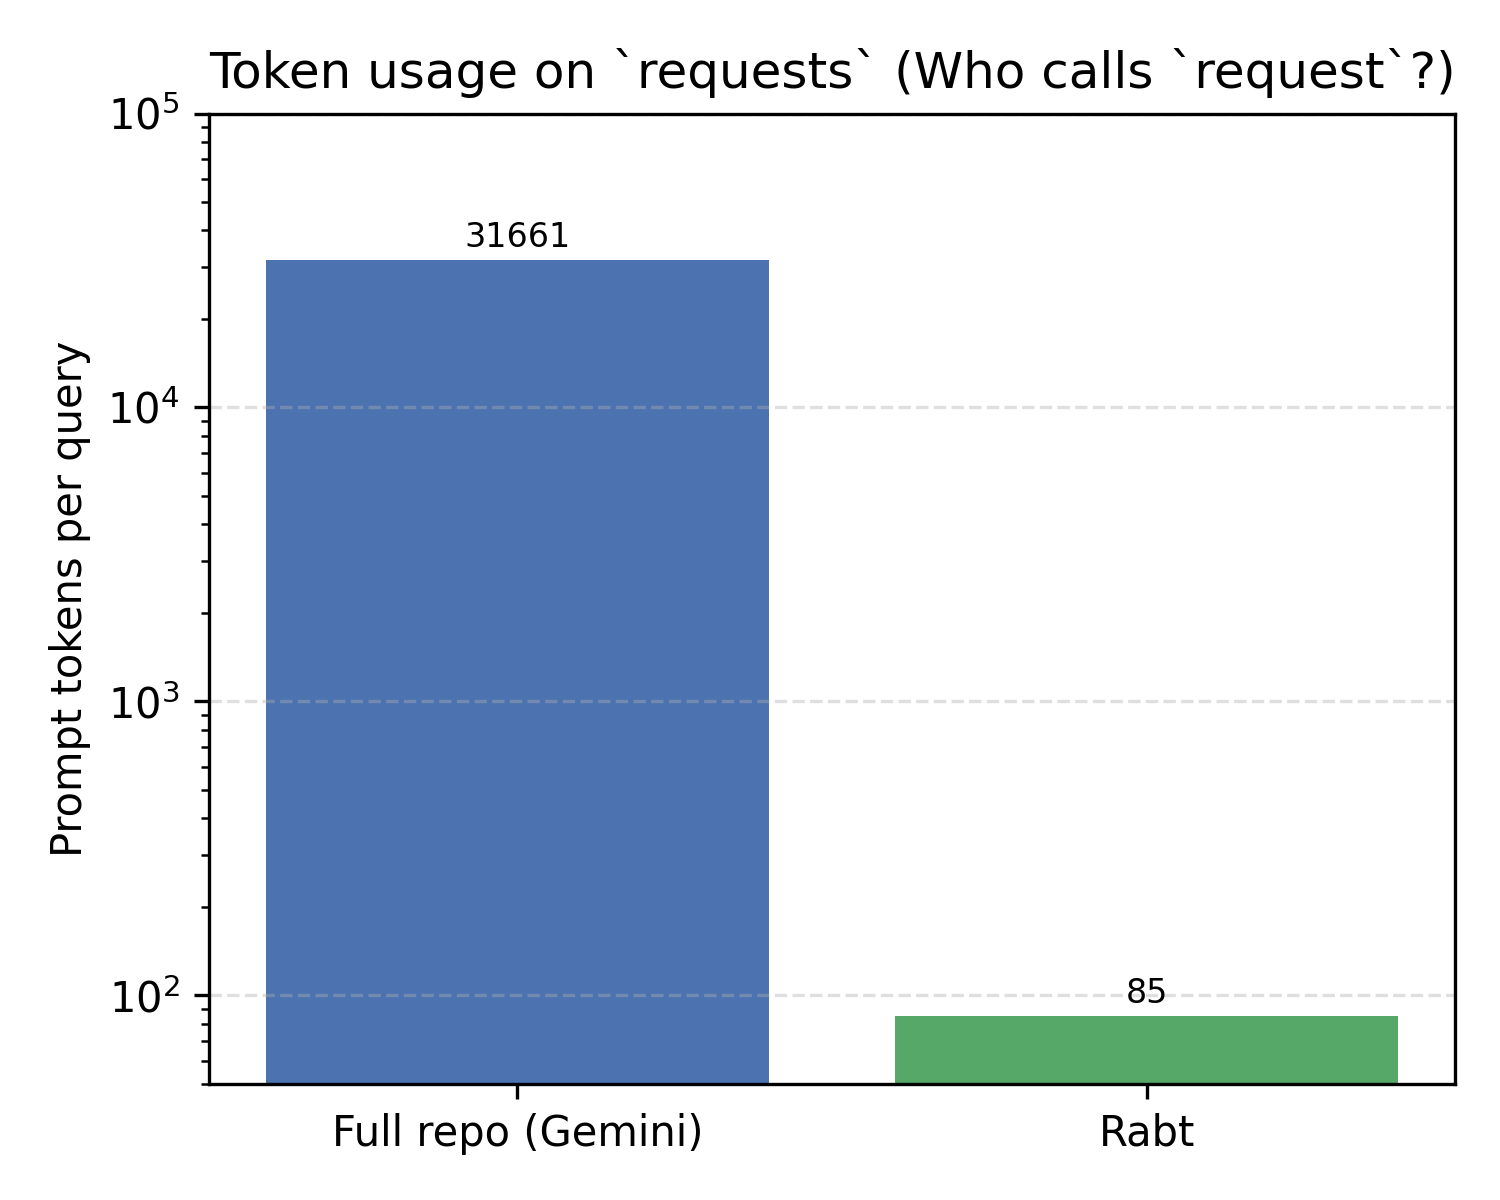
\includegraphics[width=0.6\linewidth]{plots/tokens_requests.png}
  \caption{Prompt tokens per query on the \texttt{requests} repository for the question ``Who calls \texttt{request}?''
  comparing a full-repo Gemini 2.5 Flash baseline (31{,}661 tokens) with Rabt's minimal subgraph (85 tokens), on a log scale.
  For reference, a Cursor run on the same repository and a slightly more specific prompt using Gemini 2.5 Flash consumed $\sim$14k input tokens; this value is discussed in the text but omitted from the plot for clarity.}
  \label{fig:tokens-requests}
\end{figure}

\begin{figure}[t]
  \centering
  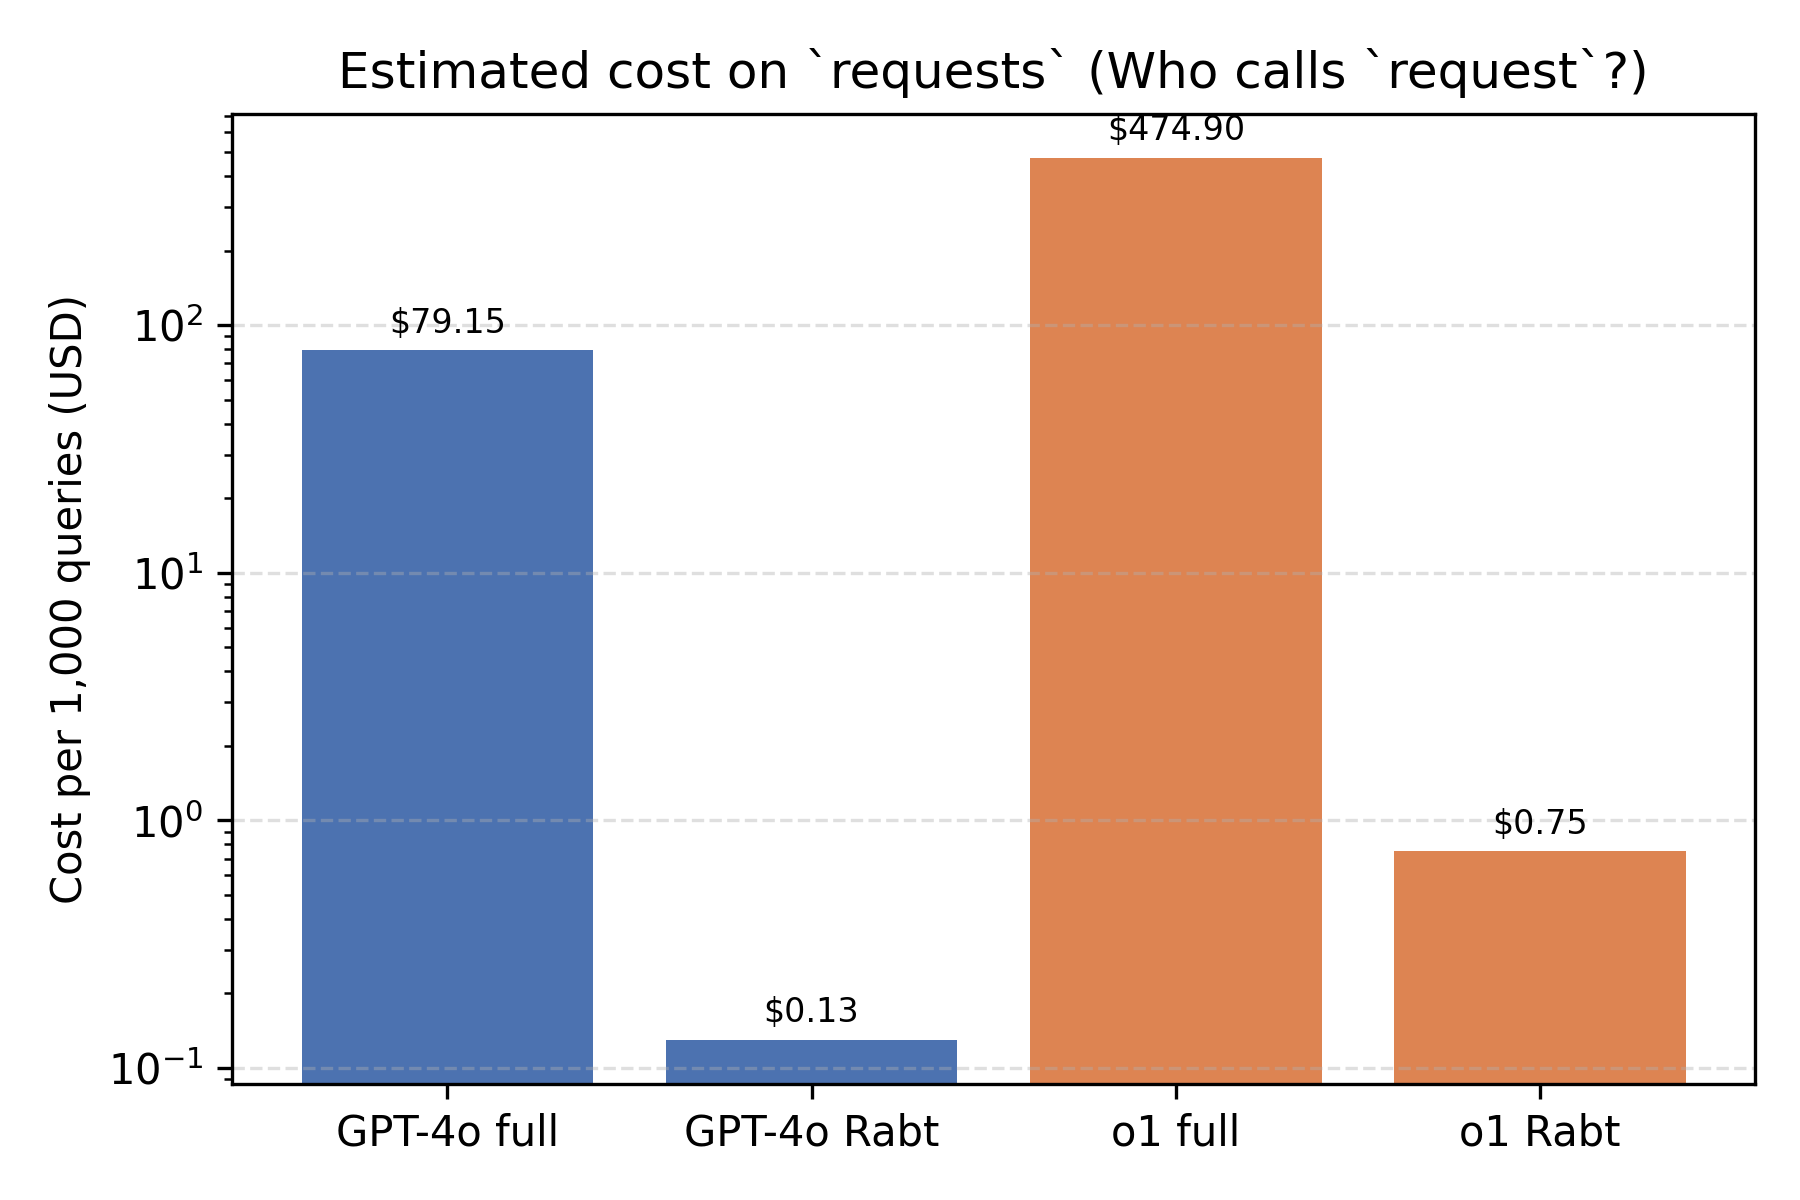
\includegraphics[width=0.6\linewidth]{plots/cost_requests.png}
  \caption{Estimated cost per 1,000 queries on \texttt{requests} under GPT-4o and OpenAI~o1 pricing.
  Using Rabt to shrink context from 31{,}661 to 85 prompt tokens reduces cost by roughly 600$\times$ while preserving answer quality.}
  \label{fig:cost-requests}
\end{figure}


\subsection{Comparison with an IDE copilot (Cursor)}

To compare Rabt with a production IDE copilot, we run the same repository and query in Cursor.
We open the \texttt{requests} codebase in Cursor, focus \texttt{src/requests/api.py}, and issue the following natural-language query in the chat:
\begin{quote}
\texttt{In this repo, who calls the function `request` in src/requests/api.py?}\\
\texttt{Please list only the function names that directly call `request()`.}
\end{quote}
Cursor answers correctly, listing the same callers as Rabt and Gemini (the public helpers \texttt{get}, \texttt{options}, \texttt{head}, \texttt{post}, \texttt{put}, \texttt{patch}, and \texttt{delete}).
From the Cursor usage dashboard we observe that this single query consumes approximately 14{,}007 new input tokens, 12{,}857 cache-read tokens, 146 output tokens, and 27{,}010 total tokens (model set to \texttt{auto}).

While Cursor's internal prompt template and retrieval heuristics are not exposed, this measurement provides a practical point of comparison: on the same codebase and question, Cursor's default behavior uses on the order of $10^4$ tokens of context, the full-repo Gemini baseline uses 31{,}661 prompt tokens, and Rabt's graph-based subgraph extraction uses only 85 prompt tokens.
Rabt therefore matches Cursor's answer quality on this query while reducing prompt size by roughly two orders of magnitude.

\subsection{Dynamic ``hidden call'' experiment}

To validate the runtime component, we construct a dynamic test where static analysis alone cannot see the call:
\begin{lstlisting}[language=Python]
from runtime.tracer import track_runtime

@track_runtime
def secret_function():
    print("I was called dynamically!")

def main():
    func_name = "secret_" + "function"
    method = globals()[func_name]
    method()  # dynamic call
\end{lstlisting}

Running the pipeline in static-only mode fails to find a clear caller for \texttt{secret\_function}.
However, after executing \texttt{dynamic\_test.py} once to generate runtime events and re-running the pipeline, Rabt correctly attributes a runtime call from the module \texttt{examples.dynamic\_test} to \texttt{secret\_function}.
This demonstrates that the hybrid static+runtime graph can recover edges that the AST alone cannot infer.

\section{Related Work}

Rabt sits at the intersection of several lines of work:
IDE copilots and context heuristics, retrieval-augmented generation for code, and graph-based models for repository-level tasks.

Commercial tools such as Cursor and GitHub Copilot maintain semantic indexes over code and use embeddings, symbol tables, and file heuristics to select context for LLMs.
They are highly optimized for user experience and broad language support, but they generally do not expose an explicit dependency graph or integrate runtime execution counts.

On the research side, Chinthareddy's study of ``Reliable Graph-RAG for Codebases'' systematically compares vector-only RAG, LLM-extracted knowledge graphs, and deterministic AST-derived graphs on Java projects, showing that deterministic syntax graphs provide better coverage and multi-hop grounding than LLM-extracted graphs at lower indexing cost~\footnote{\url{https://arxiv.org/abs/2601.08773}}.
Systems such as Microsoft's GraphRAG and open-source code-graph-rag similarly advocate graph-based memories for text and code, using Tree-sitter-derived AST graphs and knowledge graphs to answer multi-hop queries over large repositories, but they remain largely static and do not integrate lightweight runtime tracing or explicit token-level prompt minimization.
Academic work such as RepoGraph and related repository-level methods build graphs over code entities (lines, functions, classes) and use them as plug-in components for SWE-bench style systems or as inputs to graph-aware LLMs.
These methods show strong performance on benchmarks but require substantial infrastructure and often target large, real-world repositories rather than small, didactic prototypes.

Rabt differs in three key ways:
(1) it explicitly combines static and runtime edges in a single graph,
(2) it focuses on minimal subgraph extraction for context reduction and cost savings, and
(3) it implements an incremental, Git-aware graph update mechanism that makes the graph ``living''.

\section{Limitations and Future Work}

Rabt has several limitations that point to future work:
\begin{itemize}
  \item \textbf{Language and ecosystem.} The current implementation targets Python only and uses the built-in \texttt{ast} module.
  Extending to other languages would require pluggable front-ends (e.g., Tree-sitter grammars).
  \item \textbf{Partial dynamic coverage.} Runtime tracing is opt-in and function-based; dynamic constructs such as \texttt{getattr}, metaprogramming, and async code are not fully covered.
  \item \textbf{Limited evaluation scale.} Experiments focus on a sample repo and a single real-world library (\texttt{requests}), rather than full SWE-bench or CrossCodeEval benchmarks.
  \item \textbf{LLM integration.} Rabt currently serializes graphs to text and uses them as prompt context.
  Integrating the graph structure directly into the LLM's architecture, as in code graph models, is an interesting direction.
  \item \textbf{Explainability.} While subgraphs are minimal, the system does not yet provide rich natural-language explanations of why each node or edge was included.
\end{itemize}

Future work includes:
adding automated query test suites and correctness metrics;
supporting multi-language repos via Tree-sitter;
evaluating on subsets of SWE-bench Lite and CrossCodeEval;
and exploring tighter coupling between Rabt's graph and graph-aware LLMs.

\section{Conclusion}

This paper introduced Rabt, a semantic graph memory for code that combines static analysis, runtime instrumentation, impact scoring, and incremental graph updates to compute minimal dependency context for LLM-based code intelligence.
Through controlled experiments on a sample repo, a real-world library, and synthetic dynamic tests, we showed that Rabt can:
correctly answer repository-level questions;
capture runtime behaviour that pure static analysis misses; and
reduce context size by more than 99\% while preserving answer quality.

These results suggest that explicit, hybrid code graphs are a promising foundation for the next generation of AI code tools.
Instead of guessing context from file-level embeddings, systems can compute it from first principles, enabling both better reasoning and dramatically lower inference costs.

\end{document}

